% !TeX root = ../paper.tex

\section{方法}

\subsection{任务定义}

给定一个包含 $N$ 个残基的单链或多链静态结构，FlexPPI 接收氨基酸类别、主链
N--C$\alpha$--C--O 坐标以及温度、轨迹时长和数据来源等条件信息，为每个具有
有效标签的目标残基预测三类绝对动态描述符：
\begin{equation}
    \mathbf{y}_i=
    \left[y_i^{\mathrm{RMSF}},y_i^{\chi},y_i^{\mathrm{SASA}}\right]
    \in\mathbb{R}^{3}.
    \label{eq:absolute-state-target}
\end{equation}
其中 RMSF 表征主链位置涨落，$H_\chi$ 表征侧链联合旋转异构状态的多样性，SASA
表征残基溶剂暴露。状态头同时输出均值 $\hat\mu_{ik}$ 和对数方差
$\hat\ell_{ik}=\log\hat\sigma_{ik}^{2}$，下标 $k$ 对应三类指标。预测方差描述在
给定静态结构和条件后仍未被解释的残差不确定性；它与由重复轨迹或时间窗口估计的
标签方差在训练目标中分别建模。

\subsection{从分子动力学轨迹构建监督标签}

\subsubsection{数据统一与重复方差}

绝对状态预训练使用 ATLAS\cite{vandermeersche2024atlas} 和
DynaRepo\cite{mokhtari2026dynarepo}。ATLAS 提供三条重复轨迹的逐残基 RMSF；
DynaRepo 提供结构与轨迹，本文按非重叠时间窗口计算 RMSF、$H_\chi$ 和可选 SASA。
不同数据源首先被转换为统一状态记录，包括结构/轨迹路径、目标链、温度、有效时长、
来源标识及可选聚类标识。ATLAS 标签通过全局序列比对映射到结构残基；DynaRepo
要求结构与轨迹中的标准残基顺序一致，从而避免数组位置造成的残基错配。

设残基 $i$ 的某一指标具有 $M_i$ 个有效重复或窗口观测 $z_{im}$，标签均值和样本
方差定义为
\begin{equation}
    \bar z_i=\frac{1}{M_i}\sum_{m=1}^{M_i}z_{im},\qquad
    s_i^2=\frac{1}{M_i-1}\sum_{m=1}^{M_i}(z_{im}-\bar z_i)^2.
    \label{eq:label-mean-variance}
\end{equation}
当 $M_i=1$ 时记 $s_i^2=0$，表示该样本不能提供重复间方差估计，而非观测没有
噪声。每个状态分别保存 $N\times3$ 的标签均值、标签方差和有效掩码。

\subsubsection{RMSF、侧链构象熵与 SASA}

为排除整体平移和旋转，RMSF 在每条链内独立计算。对所有帧共有的 C$\alpha$
原子使用 Kabsch 算法\cite{kabsch1976solution} 将每帧对齐到参考构象。设对齐后
第 $t$ 帧的残基坐标为 $\mathbf r_{it}$，共有 $T$ 帧，则
\begin{equation}
    \bar{\mathbf r}_i=\frac{1}{T}\sum_{t=1}^{T}\mathbf r_{it},\qquad
    \mathrm{RMSF}_i=
    \sqrt{\frac{1}{T}\sum_{t=1}^{T}
    \left\|\mathbf r_{it}-\bar{\mathbf r}_i\right\|_2^2}.
    \label{eq:rmsf}
\end{equation}
DynaRepo 默认以 1,000 个保留帧组成一个非重叠窗口，并在每个窗口内独立对齐；
ATLAS 则直接汇总三条重复轨迹的预计算 RMSF。

侧链构象熵由 $\chi_1$ 至 $\chi_4$ 的联合旋转异构状态计算。每个有效扭转角被划分
为三个等宽的 $120^\circ$ 区间，残基 $i$ 在帧 $t$ 的联合状态编码为
\begin{equation}
    c_{it}=\sum_{q=1}^{Q_i}b_{iqt}3^{q-1},
    \qquad
    H_{\chi,i}=-\sum_{c:p_{ic}>0}p_{ic}\log p_{ic},
    \label{eq:chi-entropy}
\end{equation}
其中 $Q_i$ 为该残基可定义的 $\chi$ 角数，$b_{iqt}\in\{0,1,2\}$，$p_{ic}$ 为
窗口内联合状态 $c$ 的频率。本文使用自然对数且不按最大熵归一化。只有全部所需
侧链原子均存在时才计算该标签；Ala、Gly 及侧链不完整残基的 $H_\chi$ 掩码为零。

SASA 使用 Shrake--Rupley 滚球算法\cite{shrake1973environment}。本文只处理重原子，
将元素范德华半径与 $1.4$~\AA{} 水探针半径相加，并在每个原子球面使用 96 个
Fibonacci 采样点。逐原子可及面积先按残基求和，再在窗口内对帧取平均。由于该
计算需显式启用且 ATLAS 不提供 SASA，SASA 使用独立标签掩码；其缺失不影响 RMSF
和 $H_\chi$ 监督。

\subsection{FlexPPI 绝对状态网络}

\subsubsection{架构概览与逐残基输入}

图~\ref{fig:flexppi-pretraining} 概括了标签构建和状态预训练流程。FlexPPI 包含
逐残基输入分支、残基对几何分支、四层固定框架 IPA 编码器和概率状态头。一个
结构中的全部链共同构成上下文；监督掩码决定哪些残基贡献损失，非目标链仍可通过
注意力提供空间环境。

\begin{figure*}[t]
    \centering
    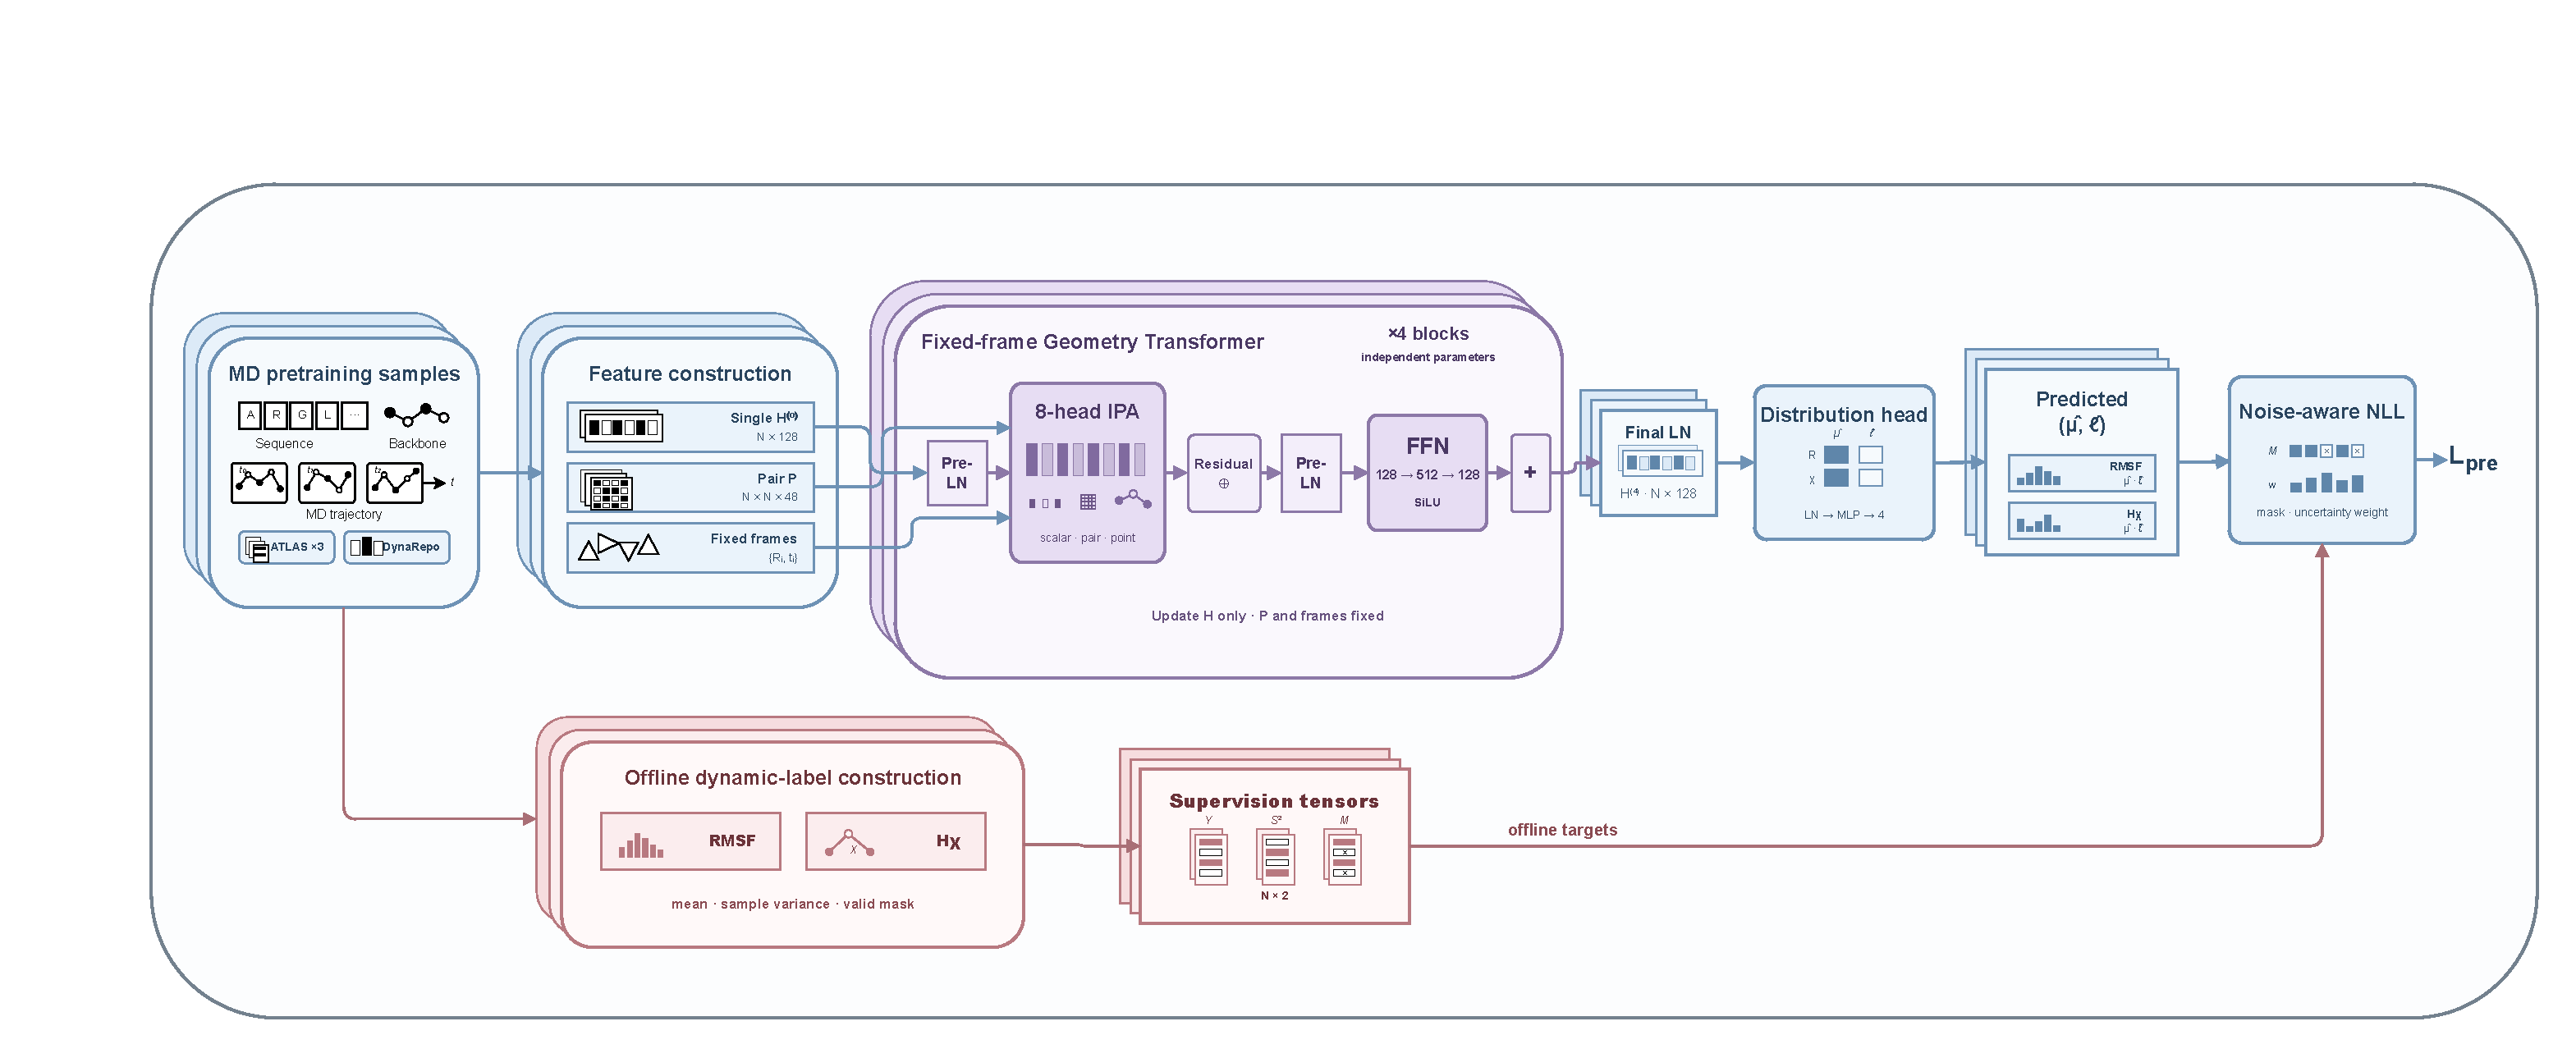
\includegraphics[width=\textwidth]{figures/f1_pipeline.pdf}
    \caption{\textbf{FlexPPI 绝对状态预训练流程。} 轨迹首先转换为逐残基 RMSF、
    侧链构象熵和 SASA 的标签均值、重复/窗口方差及有效掩码。静态结构分支构造
    氨基酸与条件表示、固定局部框架和残基对几何；四个具有独立参数的 IPA 模块在
    完整多链结构内传播标量、残基对和三维点信息。概率状态头输出三类动态量的均值
    与对数方差，并通过噪声感知负对数似然训练。}
    \label{fig:flexppi-pretraining}
\end{figure*}

当前模型使用两个独立的可学习氨基酸嵌入：主要序列嵌入
$\mathbf s_i\in\mathbb R^{128}$ 和辅助类型嵌入
$\mathbf a_i\in\mathbb R^{32}$。二者拼接并投影到 128 维。温度、轨迹时长和
数据来源组成条件向量
\begin{equation}
    \mathbf c=
    \left[\frac{T-300}{20},
    \frac{\log(1+t_{\mathrm{ns}})}{\log(501)},
    d_{\mathrm{set}}\right],
    \label{eq:condition-vector}
\end{equation}
其中 $d_{\mathrm{set}}=0$ 表示 ATLAS，$d_{\mathrm{set}}=1$ 表示 DynaRepo。
两层多层感知机将 $\mathbf c$ 映射为 128 维条件嵌入，初始残基表示为
\begin{equation}
    \mathbf h_i^{(0)}=
    \mathbf W_{\mathrm{in}}[\mathbf s_i\Vert\mathbf a_i]
    +\mathbf b_{\mathrm{in}}+\mathbf e^{\mathrm{cond}}.
    \label{eq:single-input}
\end{equation}
未知氨基酸保留为有效输入；批内填充位置和缺少有效主链框架的残基由掩码排除。

\subsubsection{固定局部框架与残基对几何}

对残基 $i$，以 C$\alpha$ 坐标为原点 $\mathbf t_i$，以 C$\alpha\rightarrow$C
方向为第一轴，将 C$\alpha\rightarrow$N 方向正交化为第二轴，并以叉乘得到第三轴，
构成旋转矩阵 $\mathbf R_i\in\mathbb R^{3\times3}$。缺少 N、C$\alpha$ 或 C 的
残基不参与几何注意力。对每个有序残基对 $(i,j)$，模型计算 C$\alpha$ 距离
$d_{ij}$、同链指示量、截断到 32 的残基编号间隔，以及在 $i$ 的局部框架中观察
$j$ 的单位方向
\begin{equation}
    \mathbf u_{ij}=
    \frac{\mathbf R_i^{\mathsf T}(\mathbf t_j-\mathbf t_i)}
    {\|\mathbf t_j-\mathbf t_i\|_2+\varepsilon}.
    \label{eq:local-direction}
\end{equation}
距离经 24 个中心均匀分布于 $0$--$24$~\AA{} 的径向基函数展开。原始几何特征
\begin{equation}
    \mathbf g_{ij}=
    \left[\boldsymbol\phi(d_{ij})\Vert
    \delta_{ij}^{\mathrm{chain}}\Vert
    \frac{\min(|r_i-r_j|,32)}{32}\Vert
    \mathbf u_{ij}\right]\in\mathbb R^{29}
    \label{eq:raw-pair-feature}
\end{equation}
由两层多层感知机投影为 $\mathbf p_{ij}\in\mathbb R^{48}$。距离和局部方向在
整体刚体变换下保持不变，因此残基对编码不依赖结构文件的全局坐标系。

\subsubsection{固定框架 IPA 与状态头}

四个 IPA 模块接收逐残基表示、残基对表示和固定框架。IPA 沿用
AlphaFold2\cite{jumper2021alphafold} 的基本构造：每个注意力头同时使用标量
查询--键相似度、残基对偏置和三维查询点--键点距离。对头 $h$，未归一化注意力
分数写为
\begin{equation}
    e_{ij}^{(h)}=
    \sqrt{\frac{1}{3d_h}}
    \langle\mathbf q_i^{(h)},\mathbf k_j^{(h)}\rangle
    +\sqrt{\frac{1}{3}}b^{(h)}(\mathbf p_{ij})
    -\frac{\gamma_h}{2}\sum_{r=1}^{P}
    \left\|
    \mathbf R_i\mathbf q_{ir}^{(h),\mathrm{pt}}+\mathbf t_i-
    \mathbf R_j\mathbf k_{jr}^{(h),\mathrm{pt}}-\mathbf t_j
    \right\|_2^2,
    \label{eq:ipa-logit}
\end{equation}
其中 $d_h=16$、$P=4$，$\gamma_h$ 为可学习的非负点距离权重。对有效残基 $j$
执行 softmax 后，注意力权重同时聚合 16 维标量值、48 维残基对值和 8 个三维
值点；三维聚合结果转换回查询残基的局部框架。每个模块包含 8 个头，并采用标准
Transformer\cite{vaswani2017attention} 的预归一化、残差连接和逐位置前馈网络。
局部框架和坐标在四层编码过程中固定，网络只更新逐残基隐藏表示。

最终状态头对 128 维残基表示执行 LayerNorm、线性变换和 SiLU 激活，输出三组
均值与对数方差。均值经 softplus 约束为非负；对数方差截断至 $[-8,6]$。因此
两个输出张量的形状均为 $N\times3$。

\subsection{噪声感知目标与训练设置}

对残基 $i$ 和指标 $k$，模型方差为 $\exp(\hat\ell_{ik})$，标签重复方差为
$s_{ik}^{2}$。二者相加后使用异方差高斯负对数似然：
\begin{equation}
    \ell_{ik}=\frac{1}{2}\left[
    \frac{(\hat\mu_{ik}-y_{ik})^2}
    {\exp(\hat\ell_{ik})+s_{ik}^{2}}
    +\log\left(\exp(\hat\ell_{ik})+s_{ik}^{2}\right)
    \right].
    \label{eq:pretraining-nll}
\end{equation}
第一项降低高噪声标签对均值误差的权重，第二项防止模型仅通过增大预测方差降低
损失。总方差截断到 $[10^{-6},10^6]$。令 $m_{ik}$ 同时表示目标残基、标签存在、
非填充和局部框架有效，则
\begin{equation}
    \mathcal L_{\mathrm{pre}}=
    \frac{\sum_{i,k}m_{ik}w_k\ell_{ik}}
    {\max(\sum_{i,k}m_{ik}w_k,1)},
    \qquad
    (w_{\mathrm{RMSF}},w_\chi,w_{\mathrm{SASA}})=(1,0.5,0.25).
    \label{eq:pretraining-loss}
\end{equation}

ATLAS 与 DynaRepo 清单合并后，划分程序依次尝试按同源簇、PDB 和样本标识分组；
当前清单缺少前两类字段，因此实际按样本标识、固定随机种子 7 划分 10\% 验证集。
该划分不是同源隔离测试，故内部结果仅作模型选择和能力诊断。预训练使用 4 层、
8 头 IPA，残基表示维度 128、残基对维度 48、dropout 0.1、批大小 1 和最大长度
768；模型训练 20 个 epoch，采用 AdamW，学习率 $3\times10^{-4}$、权重衰减
$10^{-4}$，梯度范数截断为 1.0，并保存验证损失最低的检查点。
